\section{Reuse and Warmstarting Optimizations}\label{sec-reuse-and-warmstarting}
With the experiment graph constructed and materialized, we can look for optimization opportunities for feature engineering and model training operations.
In this section, we propose two optimizations, namely, \textit{Reuse} and \textit{Warmstarting}.
Both optimizations are part of the the global optimization step of our system and can greatly reduce the execution time of a workload.

\begin{figure}
\centering
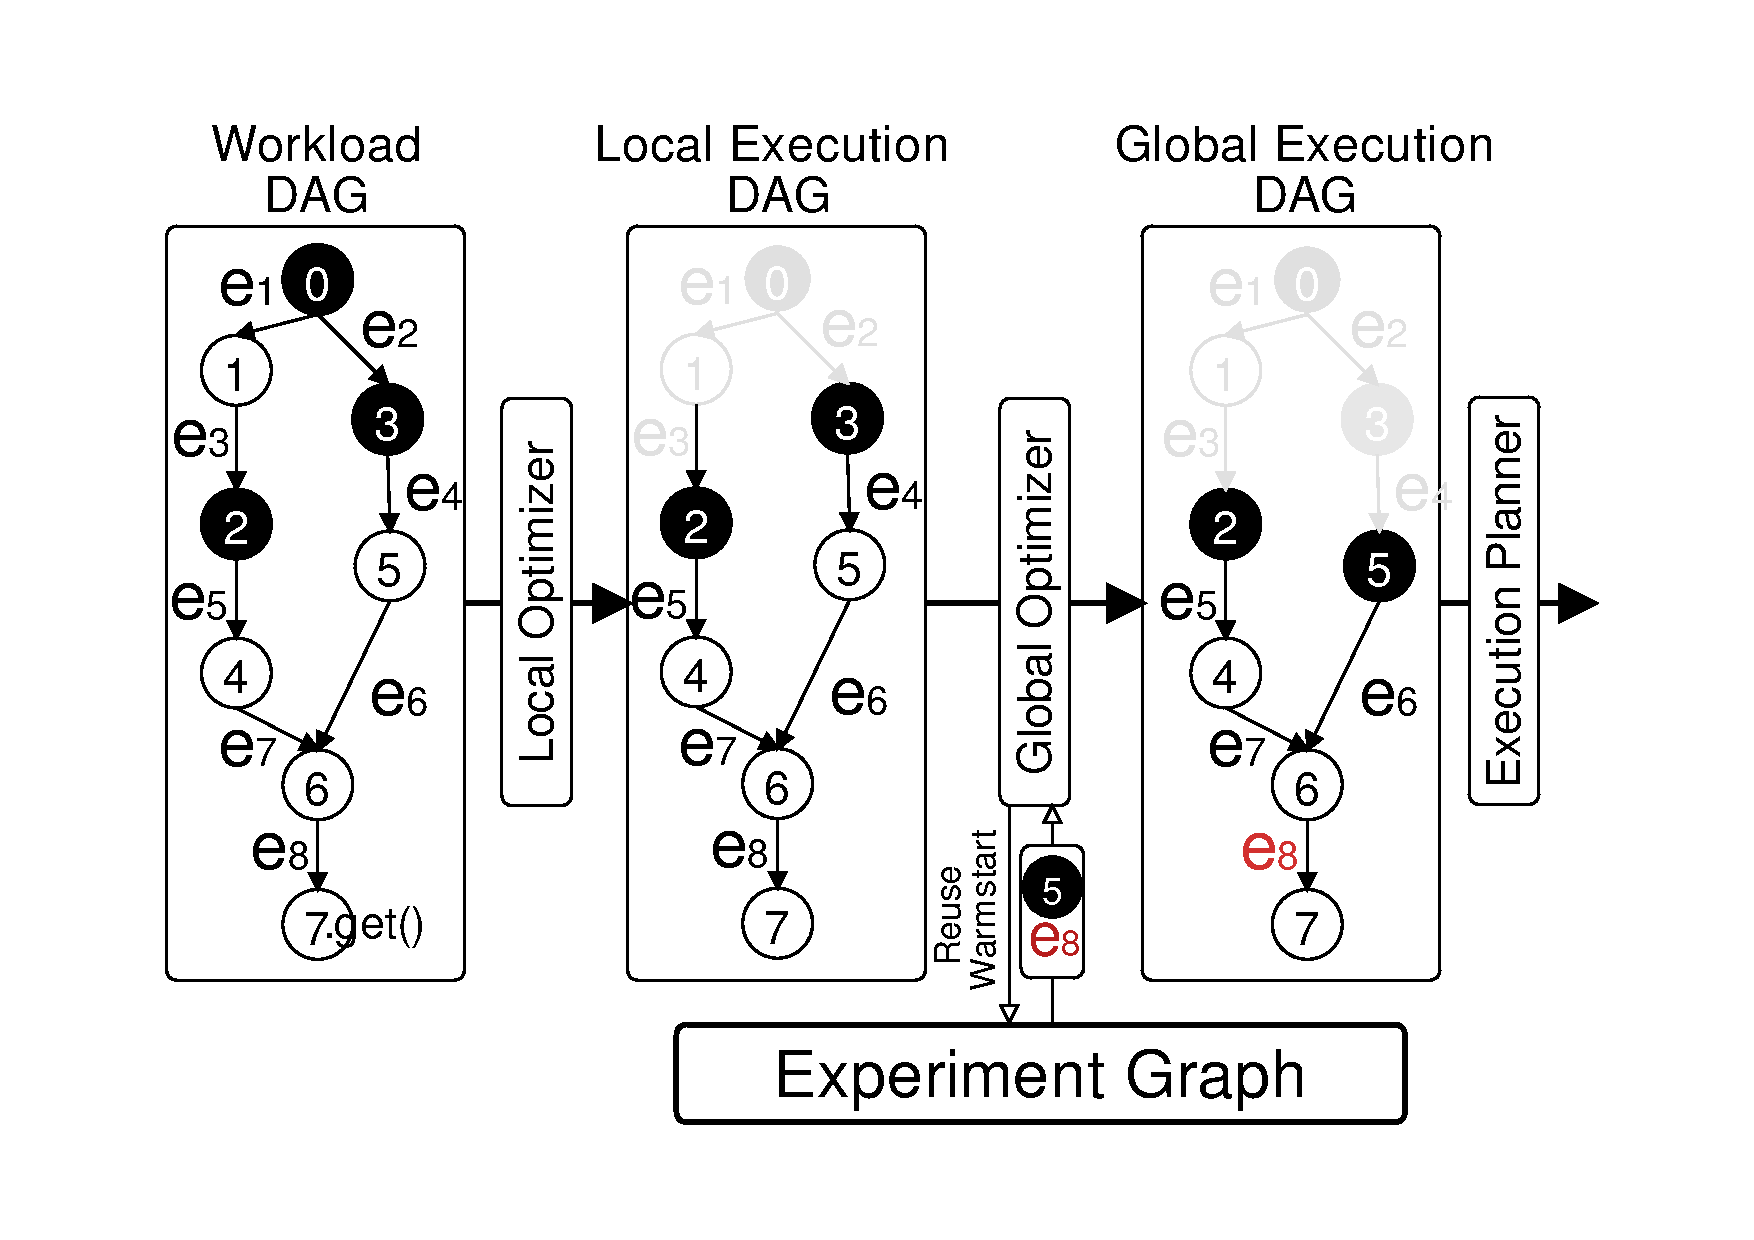
\includegraphics[width=\columnwidth]{../images/reuse-optimization}
\caption{Reuse and Warmstarting Optimizations}
\label{global-optimization}
\end{figure}
Figure \ref{global-optimization} shows an example of the optimization process for reuse.
In the workload DAG, the user invokes the $.get()$ command on vertex 7.
To compute the local execution DAG, the local optimizer scans the workload DAG for any previously computed vertices.
Besides from the root vertex (vertex 0), vertex 2 and 3 are also previously computed.
Therefore, the local optimizer prunes vertex 0 and edges $e_1$ and $e_2$.
Then, the global optimizer looks reuse opportunities in the experiment graph.
In this example, vertex 5 was computed in a previous workload and its result was materialized in the experiment graph.
During the global optimization step, the experiment graph transfers vertex 5 to the workload, which results in further pruning of vertex 3 and edge $e_4$.
In the rest of this section, we present our reuse algorithm.

\todo[inline]{Formulate Warmstarting and add a subsection.}
%Furthermore, if the workload execution subgraph contains a model training operation, the remote optimizer looks for similar models in the experiment graph, and sets the initial weight parameters of the model in the workload execution subgraph to the model in experiment graph before executing the training operation.
%This process, which is called model warmstarting, can greatly reduce the training time of machine learning models.

%Furthermore, We also look for warmstarting opportunities for any model training operations.
%The result of Step 3 is another execution subgraph with (possibly) more edges pruned.
%Finaly, we compute the execution plan using the the optimized execution subgraph (Step 4, Figure \ref{system-workflow}).

\subsection{Reuse}
Since during the materialization process, we ensure the recomputation cost of a materialized vertex outweighs its transfer cost (i.e. $trf(v) \geq rc(G,v)$), we can safely transfer the materialized vertex to the machine executing the workload and guarantee the total execution time will improve.

The global optimizer component compares the local execution DAG with the experiment graph to find any vertices that are materialized in the experiment graph and returns them instead of computing them.
The vertex hashing procedure in Section \ref{sec-ml-workloads} indicates that two vertices from two different graphs are the same if they have the same id (hash value).
%Since id of a vertex captures the exact list of proceeding operations (edges) from the root vertices, if two vertices have the same hash, they also have the same list of proceeding operations.
Therefore, to find matching vertices in the local execution DAG, global optimizer queries their ids in the experiment graph.

However, in cases where querying the experiment graph incurs a penalty, such as when the experiment graph is stored on a remote computing machine or there are many concurrent workloads being executed in the collaborative platform, we must minimize the number of queries to the experiment graph.
In this section, we present three approaches for searching the experiment graph for materialized vertices, namely, BottomUp reuse, TopDown reuse, and Hybrid reuse.

\textbf{BottomUp reuse.}
The process of BottomUp reuse is similar to how we construct the local execution DAG.
Algorithm \ref{algorithm-bottomup} shows the details of the BottomUp reuse.
The algorithm receives the local execution DAG ($G_L(V_L, E_L)$), the terminal vertex $v_t$ whose data is requested, and the experiment graph ($G_E(V_E, E_E)$).
The BottomUp reuse utilizes the following early-stopping principle. 
If a vertex from in $G_L$ exist in $G_E$ and is materialized ($is\_mat(G_E, v)$ function returns true if $v$ is materialized in $G_E$ ), then we skip traversing its parents and add the vertex to the set of materialized vertices.
Therefore, in Line 1, if $v_t$ is materialized, we return it as the result and in Lines 8-11, we only continue the search if the vertex ($v$) is not materialized.
For any other vertex which is not materialized, we recursively examine its parents until there are no more vertices left (i.e., we reach the root vertices).

\begin{algorithm}[h]
\caption{BottomUp Reuse}\label{algorithm-bottomup}
\begin{algorithmic}[1]
\Require $v_t$: terminal vertex, $G_L$: local execution DAG, $G_E$: experiment graph
\Ensure set of materialized vertices $\mathcal{M}$ 
\If {$is\_mat(G_E, v_t)$}
	\State return $\{v_t\}$
\EndIf
\State $Q \coloneqq  Queue(v_t)$  
\State $\mathcal{M} \coloneqq \emptyset$
\While {$Q.not\_empty()$}
	\State $cur  \coloneqq  Q.pop()$
	\For {$v \in parents (G_L, cur)$}
		\If {$is\_mat(G_E, v)$}
			\State	$\mathcal{M}.append(v)$
		\Else
			\State $q.add(v)$
		\EndIf
	\EndFor
\EndWhile
\State return $\mathcal{M}$
\end{algorithmic}
\end{algorithm}
BottomUp reuse performs well when the terminal vertex or vertices close to the terminal are materialized in the experiment graph.
However, in extreme cases, where none of the vertices of the local execution DAG are in the experiment graph, BottomUp reuse still has to examine all the vertices.
Therefore, BottomUp reuse has a complexity of $\mathcal{O}(|V_L|)$, where $|V_L|$ is the number of vertices in the local execution DAG, which means the global optimizer may make up to $|V_L|$ calls to the experiment graph.

\textbf{TopDown reuse.}
Contrary to the BottomUp reuse, in TopDown, we start traversing the local execution DAG, from its root vertices.

\begin{algorithm}[h]
\caption{TopDown Reuse}\label{algorithm-topdown}
\begin{algorithmic}[1]
\Require $v_t$: terminal vertex, $G_L$: local execution DAG, $G_E$: experiment graph 
\Ensure set of materialized vertices $\mathcal{M}$ 
\State $R=roots(G_L)$
\State $\mathcal{M} \coloneqq \emptyset$
\For {$r \in R$}
	\If {$r \notin G_E$}
		\State continue \Comment{skip this iteration}
	\EndIf
	\State $Q \coloneqq  Queue(r)$  
	\If {$is\_mat(G_E, r)$}
		 \State	 $\mathcal{M}.append(r)$
	\EndIf
		\While {$Q.not\_empty()$}
			\State $cur \coloneqq  Q.pop()$
			\For {$v \in children (G_L, cur)$}
				\If {$is\_mat(G_E, v)$}
					\State	$\mathcal{M}.append(v)$
				\EndIf
				\If {$v \in G_E$} 
					\State $q.add(v)$
				\EndIf
			\EndFor
		\EndWhile
\EndFor
\State return $\mathcal{M}$
\end{algorithmic}
\end{algorithm}
Algorithm \ref{algorithm-topdown} shows the details of the TopDown reuse algorithm.
The TopDown reuse operates on the following early-stopping principle.
If a vertex from $G_L$ does not exist in the experiment graph ($G_E$), we skip the traversal of its children.
This follows from the graph construction procedure, where each vertex is derived from its parents, as a result, it is impossible for a child vertex to exist in a graph where its parents do not.
Therefore, in Lines 4 and 14, we stop the traversal if the vertex is not in $G_E$.
Since a workload execution graph may have multiple root vertices, the TopDown reuse algorithm first finds all the root vertices (Line 1).
Then, for every root vertex, TopDown examines all of its children and add them to the set of materialized vertices if they are in the experiment graph and are materialized ($is\_mat$ returns true).
Unlike the BottomUp approach, when a node is materialized, we cannot stop the traversal, since a materialized vertex may also have materialized children.

TopDown performs well in scenarios where the vertices close to the root are materialized.
If the current workload operates on a completely new root (which never appeared in the experiment graph) or the workload contains early data exploration which never appeared in experiment graph, TopDown reuse will quickly stop the search process.
However, in extreme cases, where the terminal vertex is materialized in the experiment graph (i.e., a workload is re-executed), then TopDown must traverse the entire local execution DAG.
Therefore, TopDown reuse also has a complexity of $\mathcal{O}(|V_L|)$ and makes at most $|V_L|$ calls to the experiment graph.

\todo[inline]{Hybrid reuse still needs a bit of work, I'm currently implementing it to see its impact and if it is even useful}
\textbf{Hybrid reuse.}
Both BottomUp and TopDown reuse perform well in specific scenarios. 
However, neither of them can adapt to the different characteristics of a workload (e.g., how similar a new workload is to the previous workloads or how large the execution DAG is).
We devise a dynamic reuse approach, called Hybrid reuse, which adapts to the current workload.
Algorithm \ref{algorithm-hybrid} shows the process of Hybrid reuse.
Hybrid reuse combines the two early-stopping principles utilized in TopDown and BottomUp reuse algorithms to prune as many vertices without querying the experiment graph.
The two methods $R\_BFS(v, G, n)$ and $F\_BFS(v, G, n)$, perform a breadth-first-search traversal starting from vertex $v$ and return the vertex after $n$ visits.
$R\_BFS$ traverses in the reverse direction of the edges (visiting the parents of the vertex) and $F\_BFS$ traverses in along the direction of the edges (visiting children of the vertex).
It is important to emphasize that the two methods,  $R\_BFS$ and $F\_BFS$, do not make calls to the experiment graph and only return a vertex in the local execution DAG after the specified visits.

First, Hyrbid reuse traverses $G_L$ starting from the terminal node in reverse ($R\_BFS$, Line 4) until it visits half of the vertices ($|V_L|/2$).
Hybrid reuse then iteratively prunes half of the remaining vertices and adds any materialized vertex from the experiment graph to the set of materialized vertices.
In Line 7, if the vertex is not in the experiment graph, using the TopDown early-stopping principle, the algorithm prunes the bottom half of the graph and search in the top half (i.e., $R\_BFS$ on Line 8).
If the vertex is materialized (Line 16), the algorithm first adds it to the list of materialized vertices, then uses the BottomUp early-stopping principle to prune the top half the graph (i.e., $F\_BFS$ on Line 18).
When the vertex is in the experiment graph but it is not materialized (Line 9), the algorithm cannot safely prune the graph, as materialized vertices can still appear in either top half or bottom half, or both.
Hybrid reuse utilizes the following heuristic to decide which half of the graph to prune.
First, it computes the average value of the utility function for the parents and children of the vertex (Lines 10 and 11).
If the average utility of the parents is larger, then it prunes the bottom half, otherwise, it prunes the top half.
The intuition behind this heuristic is the following.
The materialization algorithm always materializes vertices based on their utility value.
Therefore, if the utility of parents of a vertex is larger than the utility of its children, then there is a higher likelihood that more vertices in the top half of the graph are materialized.

\begin{algorithm}[h]
\caption{Hybrid Reuse}\label{algorithm-hybrid}
\begin{algorithmic}[1]
\Require $v_t$: terminal vertex, $G_L$: local execution DAG, $G_E$: experiment graph
\Ensure set of materialized vertices $\mathcal{M}$ 
\State $N \coloneqq |V_L|$
\State $step \coloneqq 2$
\State $\mathcal{M} \coloneqq \emptyset$
\State $v \coloneqq R\_BFS(v_t, G_L, N/step)$
\While {$step \leq log(N) $}
		\State $step = step \times 2$
		\If {$v \notin G_E$}
				\State $v \coloneqq R\_BFS(v, G_L, N/step)$
		\ElsIf {$v \in G_E  \land \neg is\_mat(G_E,v)$}
				\State $prev \coloneqq avg (\mathcal{U}(parents(G_E v))$
				\State $next \coloneqq avg (\mathcal{U}(children(G_E, v))$
				\If{$prev \geq next $}
						 \State $v \coloneqq R\_BFS(v, G_L, N/step)$
				\Else
					\State $v \coloneqq F\_BFS(v, G_L, N/step)$
				\EndIf
		\ElsIf {$is\_math(G_E, v)$}
				\State $\mathcal{M}.append(v)$
				\State $v \coloneqq F\_BFS(v, G_L, N/step)$
		\EndIf
\EndWhile
\State return $\mathcal{M}$
\end{algorithmic}
\end{algorithm}
The advantage of the Hybrid reuse is that it requires at most $log(|V_L|)$ calls to the experiment graph since in every iteration we are pruning half of the graph.
This is in contrast to the TopDown and BottomUp reuses, wherein certain scenarios they may require $|V_L|$ calls to the experiment graph.

\subsection{Warmstarting}
Many machine learning model training operations contain random processes.
For example, in random forests, to decide when to split a node, features are randomly permuted.
Therefore, the resulting model, even on the same training data, may vary between runs.
The random behavior is controlled by a random seed parameter.
When the user does not explicitly set the random seed parameter, the result of different runs of a training operation may result in different models.
Therefore, the Reuse algorithm is not able to find the previously trained model, even if all the other hyperparameters (except for random seed) are the same.

Many machine learning training algorithms first initialize the model parameters before the training begins. 
Warmstarting is a technique, in which the model parameters are set to a previously trained model which decreases the total training time \cite{baylor2017tfx}.
In the presence of different random seed parameters, we rely on warmstarting to decrease the execution time of a training operation.
The process of warmstarting in the experiment graph is as follows.
During the graph construction, for machine learning model training operations, apart from the hash value which takes into account all the hyperparameters, we also compute another hash which does not consider the random seed parameter, we refer to this hash value as the warmstarting hash.
When the Reuse algorithm encounters a machine learning model node, one of the three followings occurs.
In the first case, the machine learning model node also exists in the experiment graph. 
This indicates apart from all the hyperparameters the random seed parameters of the training operation in the experiment graph and the workload graph were the same.
In this case, we can safely reuse the model.
In the second case, the machine learning model node does not exist in the experiment graph, but the parent vertex (the training data node) and an edge with the same warmstarting hash exist in the experiment graph.
In this case, the model vertex from the experiment graph is selected as a warmstarting candidate.
If there are more than one warmstarting candidates, the model vertex with the highest score is used for warmstarting.
In the third case, neither the model vertex nor its parent node is in the experiment graph.
In this case, no reuse or warmstarting is possible.



